\subsection{Bubble Sort}

\subsubsection{Core concept}
Bubble sort is also comparison-based sorting algorithm. The bubble sort compares adjacent items and exchanges them if they are out of order. This sort usually requires several passes over the data. ~\cite{ref7}

\vspace{5pt}

\subsubsection{Explanation}
\textbf{One way to explain this algorithm:}

Traverse from left and compare adjacent elements and the higher one is placed at right side. In this way, the largest element is moved to the rightmost end at first. This process is then continued to find the second largest and place it and so on until the data is sorted. ~\cite{ref9}

\vspace{5pt}

Lets consider the following array as an example: {29, 10, 14, 37, 13} ~\cite{ref7} 

\vspace{5pt}

\textbf{The first pass: }
Compare the items in the first pair 29 and 10 and exchange them because they are out of order. Next you consider the second pair 29 and 14 and exchange these items because they are out of order. The items in the third pair 29 and 37 are in order, and so you do not exchange them. Finally, you exchange the items in the last pair 37 and 13.

\vspace{5pt}

\textbf{The second pass:}
During the second pass of the bubble sort, return to the beginning of the array and consider pairs of items in exactly the same manner as the first pass. Do not, however, include the last and largest—item of the array. That is, the second pass considers the first n – 1 items of the array. After the second pass, the second-largest item in the array will be in its proper place in the next-to-last position of the array.

Now, ignoring the last two items, which are in order, continue with subsequent passes until the array is sorted.

The first two passes of a bubble sort of an array of five integers ~\cite{ref7}

\vspace{5pt}

\subsubsection{Complexity analysis}
\textbf{Time complexity:}
In each iteration of variable \(i\), the smallest element in the segment \(a[i \ldots n-1]\) will "bubble up" and be placed at \(a[i]\). Therefore, there are a total of \((n-1)\) iterations for variable \(i\).

Iteration 1: there are \((n-1)\) comparisons between \(a[j]\) and \(a[j-1]\), with \(j\) going from \(n-1\) to 1.

Iteration 2: there are \((n-2)\) comparisons between \(a[j]\) and \(a[j-1]\), with \(j\) going from \(n-2\) to 1.

...

Iteration \(n-1\): there is 1 comparison between \(a[1]\) and \(a[0]\).

Let \(f(n)\) be the number of comparisons and also the number of basic operations of the Bubble Sort algorithm, we have:

\[ f(n) = (n-1) + (n-2) + \ldots + 2 + 1 = \frac{n(n-1)}{2} \]

regardless of the distribution of the array elements.
\begin{itemize}
    \item Best case: $O(n)$ - Occurs when the original data is already sorted, it uses one pass, during which n – 1 comparisons and no exchanges occur. ~\cite{ref7}
    \item Average case: $O(n^2)$ - The algorithm always performs n-1 passes and involves n(n-1)/2 comparisons on average.
    \item Worst case: $O(n^2)$ - This occurs when the list is sorted in reverse order, requiring the maximum number of swaps.
\end{itemize}

\textbf{Space complexity:} $O(1)$ – Bubble sort is an in-place sorting algorithm, meaning it requires only a constant amount of additional memory space.

\vspace{5pt}

\subsubsection{Variants and optimizations}
\begin{itemize}[label=-]
    \item One common optimization is to introduce a flag that checks whether any swaps were made during a pass. If no swaps were made, the list is already sorted, and the algorithm can terminate early, improving the best-case time complexity to $O(n)$.
    \item Shaker sort is an extension of bubble sort, we will also discuss it later. It sorts in both directions in each pass through the list. By doing so, it can more quickly bring small values to the beginning and large values to the end, which helps reduce the number of passes needed compared to standard bubble sort.
\end{itemize}

\begin{figure}[h]
    \centering
    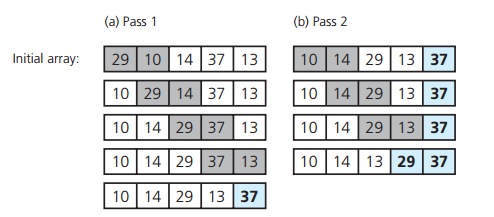
\includegraphics[scale=.80]{Figures/sort_demo/bubble.png}
    \caption{Bubble Sort Demo}
    \label{fig:enter-label}
\end{figure}

\vspace{10pt}